\documentclass[1p]{elsarticle_modified}
%\bibliographystyle{elsarticle-num}

%\usepackage[colorlinks]{hyperref}
%\usepackage{abbrmath_seonhwa} %\Abb, \Ascr, \Acal ,\Abf, \Afrak
\usepackage{amsfonts}
\usepackage{amssymb}
\usepackage{amsmath}
\usepackage{amsthm}
\usepackage{scalefnt}
\usepackage{amsbsy}
\usepackage{kotex}
\usepackage{caption}
\usepackage{subfig}
\usepackage{color}
\usepackage{graphicx}
\usepackage{xcolor} %% white, black, red, green, blue, cyan, magenta, yellow
\usepackage{float}
\usepackage{setspace}
\usepackage{hyperref}

\usepackage{tikz}
\usetikzlibrary{arrows}

\usepackage{multirow}
\usepackage{array} % fixed length table
\usepackage{hhline}

%%%%%%%%%%%%%%%%%%%%%
\makeatletter
\renewcommand*\env@matrix[1][\arraystretch]{%
	\edef\arraystretch{#1}%
	\hskip -\arraycolsep
	\let\@ifnextchar\new@ifnextchar
	\array{*\c@MaxMatrixCols c}}
\makeatother %https://tex.stackexchange.com/questions/14071/how-can-i-increase-the-line-spacing-in-a-matrix
%%%%%%%%%%%%%%%

\usepackage[normalem]{ulem}

\newcommand{\msout}[1]{\ifmmode\text{\sout{\ensuremath{#1}}}\else\sout{#1}\fi}
%SOURCE: \msout is \stkout macro in https://tex.stackexchange.com/questions/20609/strikeout-in-math-mode

\newcommand{\cancel}[1]{
	\ifmmode
	{\color{red}\msout{#1}}
	\else
	{\color{red}\sout{#1}}
	\fi
}

\newcommand{\add}[1]{
	{\color{blue}\uwave{#1}}
}

\newcommand{\replace}[2]{
	\ifmmode
	{\color{red}\msout{#1}}{\color{blue}\uwave{#2}}
	\else
	{\color{red}\sout{#1}}{\color{blue}\uwave{#2}}
	\fi
}

\newcommand{\Sol}{\mathcal{S}} %segment
\newcommand{\D}{D} %diagram
\newcommand{\A}{\mathcal{A}} %arc


%%%%%%%%%%%%%%%%%%%%%%%%%%%%%5 test

\def\sl{\operatorname{\textup{SL}}(2,\Cbb)}
\def\psl{\operatorname{\textup{PSL}}(2,\Cbb)}
\def\quan{\mkern 1mu \triangleright \mkern 1mu}

\theoremstyle{definition}
\newtheorem{thm}{Theorem}[section]
\newtheorem{prop}[thm]{Proposition}
\newtheorem{lem}[thm]{Lemma}
\newtheorem{ques}[thm]{Question}
\newtheorem{cor}[thm]{Corollary}
\newtheorem{defn}[thm]{Definition}
\newtheorem{exam}[thm]{Example}
\newtheorem{rmk}[thm]{Remark}
\newtheorem{alg}[thm]{Algorithm}

\newcommand{\I}{\sqrt{-1}}
\begin{document}

%\begin{frontmatter}
%
%\title{Boundary parabolic representations of knots up to 8 crossings}
%
%%% Group authors per affiliation:
%\author{Yunhi Cho} 
%\address{Department of Mathematics, University of Seoul, Seoul, Korea}
%\ead{yhcho@uos.ac.kr}
%
%
%\author{Seonhwa Kim} %\fnref{s_kim}}
%\address{Center for Geometry and Physics, Institute for Basic Science, Pohang, 37673, Korea}
%\ead{ryeona17@ibs.re.kr}
%
%\author{Hyuk Kim}
%\address{Department of Mathematical Sciences, Seoul National University, Seoul 08826, Korea}
%\ead{hyukkim@snu.ac.kr}
%
%\author{Seokbeom Yoon}
%\address{Department of Mathematical Sciences, Seoul National University, Seoul, 08826,  Korea}
%\ead{sbyoon15@snu.ac.kr}
%
%\begin{abstract}
%We find all boundary parabolic representation of knots up to 8 crossings.
%
%\end{abstract}
%\begin{keyword}
%    \MSC[2010] 57M25 
%\end{keyword}
%
%\end{frontmatter}

%\linenumbers
%\tableofcontents
%
\newcommand\colored[1]{\textcolor{white}{\rule[-0.35ex]{0.8em}{1.4ex}}\kern-0.8em\color{red} #1}%
%\newcommand\colored[1]{\textcolor{white}{ #1}\kern-2.17ex	\textcolor{white}{ #1}\kern-1.81ex	\textcolor{white}{ #1}\kern-2.15ex\color{red}#1	}

{\Large $\underline{11n_{164}~(K11n_{164})}$}

\setlength{\tabcolsep}{10pt}
\renewcommand{\arraystretch}{1.6}
\vspace{1cm}\begin{tabular}{m{100pt}>{\centering\arraybackslash}m{274pt}}
\multirow{5}{120pt}{
	\centering
	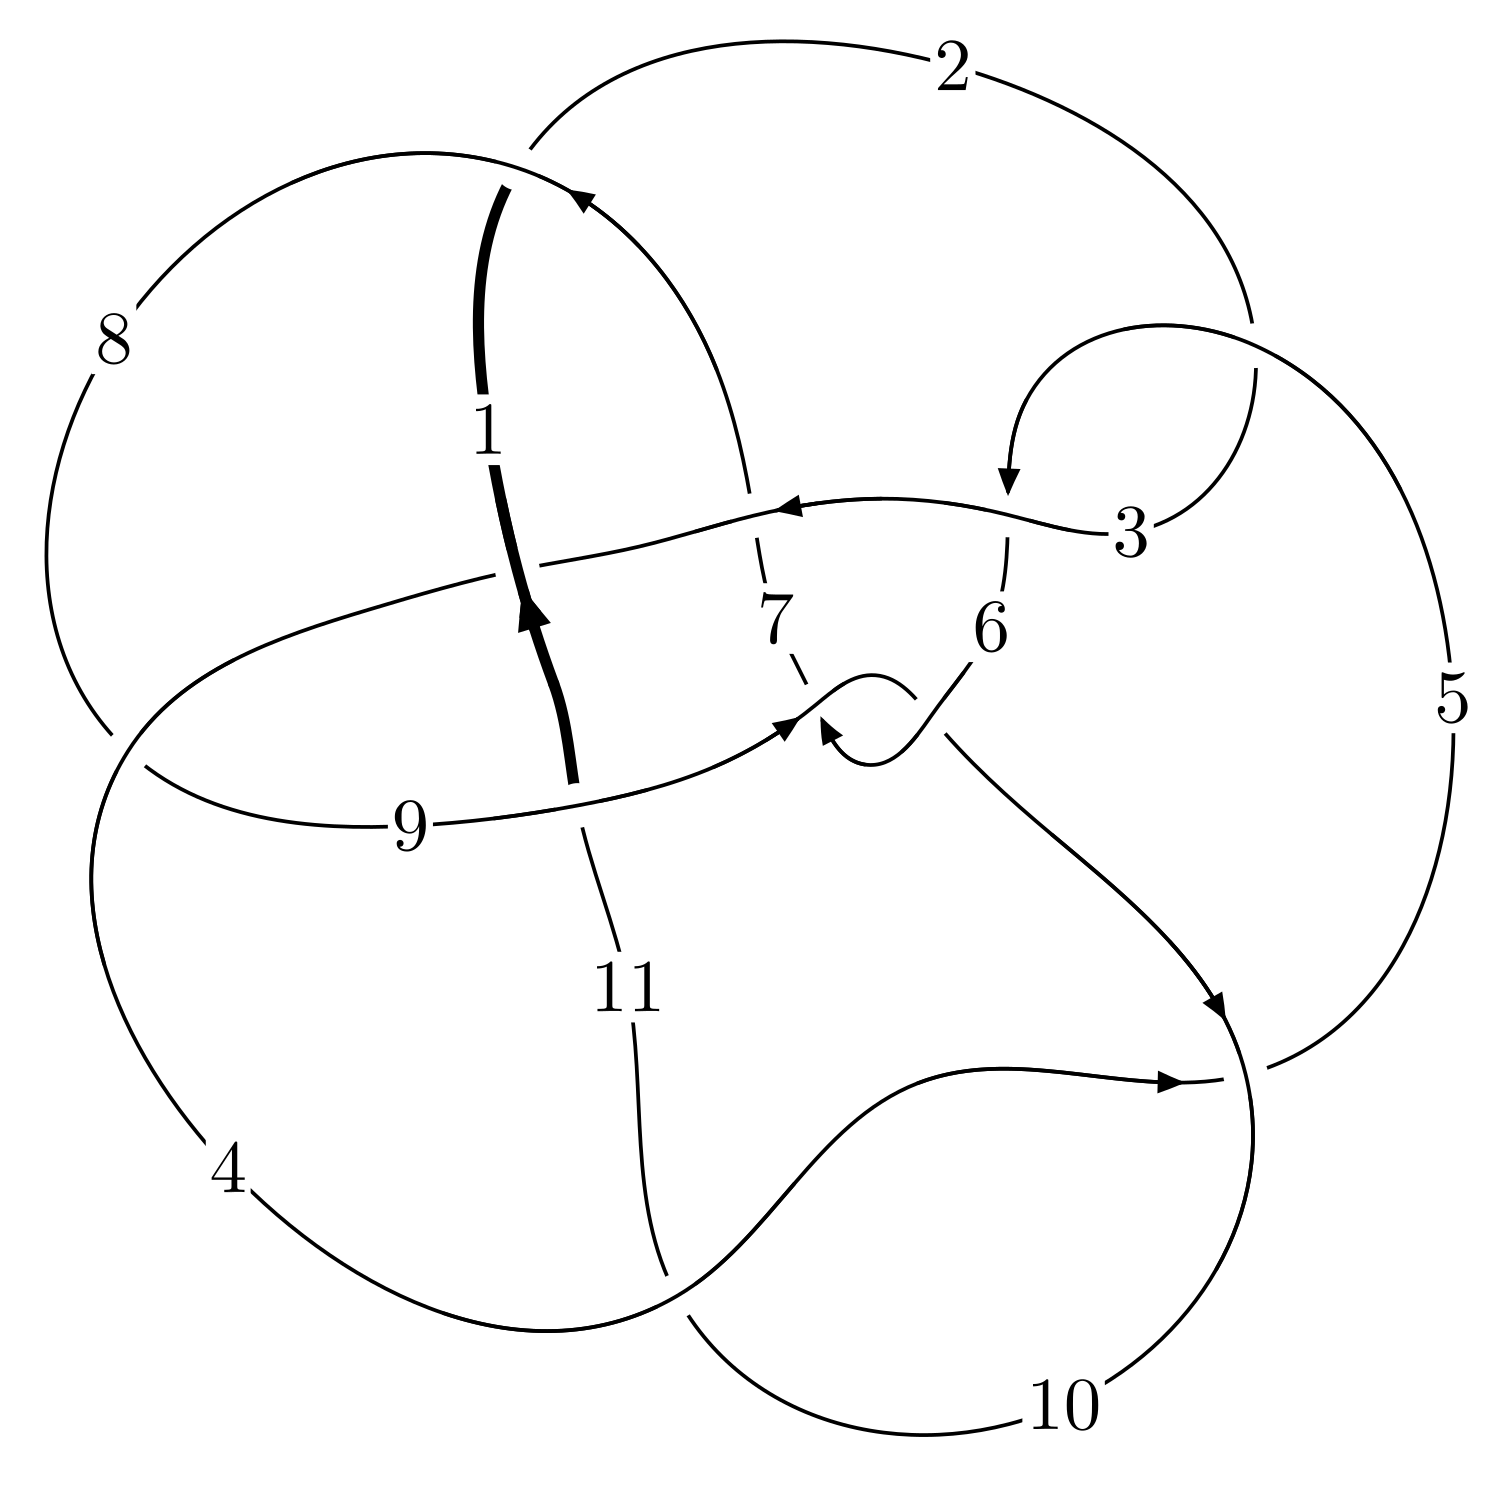
\includegraphics[width=112pt]{../../../GIT/diagram.site/Diagrams/png/780_11n_164.png}\\
\ \ \ A knot diagram\footnotemark}&
\allowdisplaybreaks
\textbf{Linearized knot diagam} \\
\cline{2-2}
 &
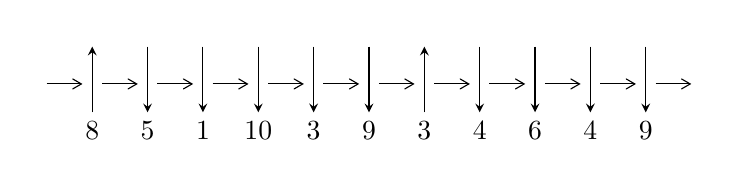
\begin{tikzpicture}[x=20pt, y=17pt]
	% nodes
	\node (C0) at (0, 0) {};
	\node (C1) at (1, 0) {};
	\node (C1U) at (1, +1) {};
	\node (C1D) at (1, -1) {8};

	\node (C2) at (2, 0) {};
	\node (C2U) at (2, +1) {};
	\node (C2D) at (2, -1) {5};

	\node (C3) at (3, 0) {};
	\node (C3U) at (3, +1) {};
	\node (C3D) at (3, -1) {1};

	\node (C4) at (4, 0) {};
	\node (C4U) at (4, +1) {};
	\node (C4D) at (4, -1) {10};

	\node (C5) at (5, 0) {};
	\node (C5U) at (5, +1) {};
	\node (C5D) at (5, -1) {3};

	\node (C6) at (6, 0) {};
	\node (C6U) at (6, +1) {};
	\node (C6D) at (6, -1) {9};

	\node (C7) at (7, 0) {};
	\node (C7U) at (7, +1) {};
	\node (C7D) at (7, -1) {3};

	\node (C8) at (8, 0) {};
	\node (C8U) at (8, +1) {};
	\node (C8D) at (8, -1) {4};

	\node (C9) at (9, 0) {};
	\node (C9U) at (9, +1) {};
	\node (C9D) at (9, -1) {6};

	\node (C10) at (10, 0) {};
	\node (C10U) at (10, +1) {};
	\node (C10D) at (10, -1) {4};

	\node (C11) at (11, 0) {};
	\node (C11U) at (11, +1) {};
	\node (C11D) at (11, -1) {9};
	\node (C12) at (12, 0) {};

	% arrows
	\draw[->,>={angle 60}]
	(C0) edge (C1) (C1) edge (C2) (C2) edge (C3) (C3) edge (C4) (C4) edge (C5) (C5) edge (C6) (C6) edge (C7) (C7) edge (C8) (C8) edge (C9) (C9) edge (C10) (C10) edge (C11) (C11) edge (C12) ;	\draw[->,>=stealth]
	(C1D) edge (C1U) (C2U) edge (C2D) (C3U) edge (C3D) (C4U) edge (C4D) (C5U) edge (C5D) (C6U) edge (C6D) (C7D) edge (C7U) (C8U) edge (C8D) (C9U) edge (C9D) (C10U) edge (C10D) (C11U) edge (C11D) ;
	\end{tikzpicture} \\
\hhline{~~} \\& 
\textbf{Solving Sequence} \\ \cline{2-2} 
 &
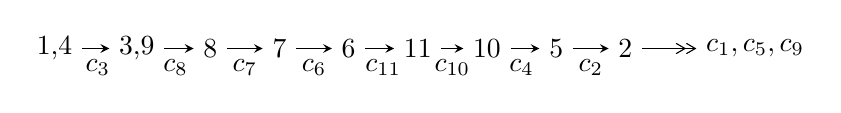
\begin{tikzpicture}[x=25pt, y=7pt]
	% node
	\node (A0) at (-1/8, 0) {1,4};
	\node (A1) at (17/16, 0) {3,9};
	\node (A2) at (17/8, 0) {8};
	\node (A3) at (25/8, 0) {7};
	\node (A4) at (33/8, 0) {6};
	\node (A5) at (41/8, 0) {11};
	\node (A6) at (49/8, 0) {10};
	\node (A7) at (57/8, 0) {5};
	\node (A8) at (65/8, 0) {2};
	\node (C1) at (1/2, -1) {$c_{3}$};
	\node (C2) at (13/8, -1) {$c_{8}$};
	\node (C3) at (21/8, -1) {$c_{7}$};
	\node (C4) at (29/8, -1) {$c_{6}$};
	\node (C5) at (37/8, -1) {$c_{11}$};
	\node (C6) at (45/8, -1) {$c_{10}$};
	\node (C7) at (53/8, -1) {$c_{4}$};
	\node (C8) at (61/8, -1) {$c_{2}$};
	\node (A9) at (10, 0) {$c_{1},c_{5},c_{9}$};

	% edge
	\draw[->,>=stealth]	
	(A0) edge (A1) (A1) edge (A2) (A2) edge (A3) (A3) edge (A4) (A4) edge (A5) (A5) edge (A6) (A6) edge (A7) (A7) edge (A8) ;
	\draw[->>,>={angle 60}]	
	(A8) edge (A9);
\end{tikzpicture} \\ 

\end{tabular} \\

\footnotetext{
The image of knot diagram is generated by the software ``\textbf{Draw programme}" developed by Andrew Bartholomew(\url{http://www.layer8.co.uk/maths/draw/index.htm\#Running-draw}), where we modified some parts for our purpose(\url{https://github.com/CATsTAILs/LinksPainter}).
}\phantom \\ \newline 
\centering \textbf{Ideals for irreducible components\footnotemark of $X_{\text{par}}$} 
 
\begin{align*}
I^u_{1}&=\langle 
- u^6+u^5-2 u^4-2 u^2+b-2 u-1,\;- u^7+3 u^6-3 u^5+2 u^4+2 u^3- u^2+3 a+6 u+3,\\
\phantom{I^u_{1}}&\phantom{= \langle  }u^8-3 u^7+6 u^6-5 u^5+4 u^4+u^3+3 u+3\rangle \\
I^u_{2}&=\langle 
-2 u^9+10 u^8-24 u^7+38 u^6-49 u^5+52 u^4-32 u^3- u^2+b+14 u-5,\\
\phantom{I^u_{2}}&\phantom{= \langle  }5 u^9-23 u^8+55 u^7-86 u^6+112 u^5-116 u^4+73 u^3+2 u^2+a-29 u+11,\\
\phantom{I^u_{2}}&\phantom{= \langle  }u^{10}-5 u^9+13 u^8-22 u^7+30 u^6-33 u^5+25 u^4-6 u^3-6 u^2+5 u-1\rangle \\
I^u_{3}&=\langle 
- u^5-2 u^4-4 u^3-3 u^2+b-2 u+1,\;- u^9-4 u^8-11 u^7-19 u^6-25 u^5-22 u^4-14 u^3-5 u^2+a- u-1,\\
\phantom{I^u_{3}}&\phantom{= \langle  }u^{10}+4 u^9+11 u^8+19 u^7+25 u^6+21 u^5+12 u^4+u^3-2 u^2- u+1\rangle \\
I^u_{4}&=\langle 
-3 u^3- a u-5 u^2+b-3 u+4,\;4 u^3 a+7 u^2 a+u^3+a^2+5 a u+2 u^2-5 a+u-2,\;u^4+u^3-2 u+1\rangle \\
I^u_{5}&=\langle 
- a u+b+u+1,\;a^2+a u-2 u-1,\;u^2+u+1\rangle \\
I^u_{6}&=\langle 
b-2,\;a+1,\;u+1\rangle \\
I^u_{7}&=\langle 
b+1,\;a-2,\;u+1\rangle \\
I^u_{8}&=\langle 
b-1,\;a+1,\;u+1\rangle \\
\\
I^v_{1}&=\langle 
a,\;b-1,\;v-1\rangle \\
\end{align*}
\raggedright * 9 irreducible components of $\dim_{\mathbb{C}}=0$, with total 44 representations.\\
\footnotetext{All coefficients of polynomials are rational numbers. But the coefficients are sometimes approximated in decimal forms when there is not enough margin.}
\newpage
\renewcommand{\arraystretch}{1}
\centering \section*{I. $I^u_{1}= \langle - u^6+u^5-2 u^4-2 u^2+b-2 u-1,\;- u^7+3 u^6+\cdots+3 a+3,\;u^8-3 u^7+6 u^6-5 u^5+4 u^4+u^3+3 u+3 \rangle$}
\flushleft \textbf{(i) Arc colorings}\\
\begin{tabular}{m{7pt} m{180pt} m{7pt} m{180pt} }
\flushright $a_{1}=$&$\begin{pmatrix}0\\u\end{pmatrix}$ \\
\flushright $a_{4}=$&$\begin{pmatrix}1\\0\end{pmatrix}$ \\
\flushright $a_{3}=$&$\begin{pmatrix}1\\- u^2\end{pmatrix}$ \\
\flushright $a_{9}=$&$\begin{pmatrix}\frac{1}{3} u^7- u^6+\cdots-2 u-1\\u^6- u^5+2 u^4+2 u^2+2 u+1\end{pmatrix}$ \\
\flushright $a_{8}=$&$\begin{pmatrix}\frac{1}{3} u^7+\frac{4}{3} u^4-\frac{2}{3} u^3+\frac{7}{3} u^2\\u^6- u^5+2 u^4+2 u^2+2 u+1\end{pmatrix}$ \\
\flushright $a_{7}=$&$\begin{pmatrix}-\frac{2}{3} u^7+2 u^6+\cdots+2 u+2\\- u^7- u^5-2 u^4-3 u^3-3 u^2-4 u-2\end{pmatrix}$ \\
\flushright $a_{6}=$&$\begin{pmatrix}-\frac{2}{3} u^7+u^6+\cdots-\frac{2}{3} u^2+1\\- u^6+u^5-2 u^4- u^3- u^2-3 u-2\end{pmatrix}$ \\
\flushright $a_{11}=$&$\begin{pmatrix}-\frac{1}{3} u^7-\frac{4}{3} u^4+\cdots-\frac{4}{3} u^2- u\\u^7-2 u^6+3 u^5- u^4+u^3+u^2-1\end{pmatrix}$ \\
\flushright $a_{10}=$&$\begin{pmatrix}\frac{2}{3} u^7-2 u^6+\cdots- u-1\\u^7-2 u^6+3 u^5- u^4+u^3+u^2-1\end{pmatrix}$ \\
\flushright $a_{5}=$&$\begin{pmatrix}-\frac{2}{3} u^7+2 u^6+\cdots+2 u+2\\-2 u^7+3 u^6-4 u^5-2 u^3-2 u^2+1\end{pmatrix}$ \\
\flushright $a_{2}=$&$\begin{pmatrix}\frac{2}{3} u^7- u^6+\cdots+u+1\\u^6- u^5+2 u^4+u^3+2 u^2+4 u+2\end{pmatrix}$\\ \flushright $a_{2}=$&$\begin{pmatrix}\frac{2}{3} u^7- u^6+\cdots+u+1\\u^6- u^5+2 u^4+u^3+2 u^2+4 u+2\end{pmatrix}$\\&\end{tabular}
\flushleft \textbf{(ii) Obstruction class $= -1$}\\~\\
\flushleft \textbf{(iii) Cusp Shapes $= -2 u^7+6 u^6-12 u^5+12 u^4-8 u^3+2 u^2-6$}\\~\\
\newpage\renewcommand{\arraystretch}{1}
\flushleft \textbf{(iv) u-Polynomials at the component}\newline \\
\begin{tabular}{m{50pt}|m{274pt}}
Crossings & \hspace{64pt}u-Polynomials at each crossing \\
\hline $$\begin{aligned}c_{1}\end{aligned}$$&$\begin{aligned}
&u^8- u^7+9 u^6-4 u^5+26 u^4-2 u^3+28 u^2+10
\end{aligned}$\\
\hline $$\begin{aligned}c_{2},c_{5},c_{8}\\c_{11}\end{aligned}$$&$\begin{aligned}
&u^8- u^7-4 u^6+5 u^5+4 u^4-3 u^3+4 u^2- u+1
\end{aligned}$\\
\hline $$\begin{aligned}c_{3},c_{6},c_{9}\end{aligned}$$&$\begin{aligned}
&u^8-3 u^7+6 u^6-5 u^5+4 u^4+u^3+3 u+3
\end{aligned}$\\
\hline $$\begin{aligned}c_{4},c_{10}\end{aligned}$$&$\begin{aligned}
&u^8+6 u^7+20 u^6+42 u^5+68 u^4+82 u^3+74 u^2+32 u+8
\end{aligned}$\\
\hline $$\begin{aligned}c_{7}\end{aligned}$$&$\begin{aligned}
&u^8+2 u^7+9 u^6+10 u^5+31 u^4+30 u^3+27 u^2+26 u+12
\end{aligned}$\\
\hline
\end{tabular}\\~\\
\newpage\renewcommand{\arraystretch}{1}
\flushleft \textbf{(v) Riley Polynomials at the component}\newline \\
\begin{tabular}{m{50pt}|m{274pt}}
Crossings & \hspace{64pt}Riley Polynomials at each crossing \\
\hline $$\begin{aligned}c_{1}\end{aligned}$$&$\begin{aligned}
&y^8+17 y^7+\cdots+560 y+100
\end{aligned}$\\
\hline $$\begin{aligned}c_{2},c_{5},c_{8}\\c_{11}\end{aligned}$$&$\begin{aligned}
&y^8-9 y^7+34 y^6-55 y^5+14 y^4+25 y^3+18 y^2+7 y+1
\end{aligned}$\\
\hline $$\begin{aligned}c_{3},c_{6},c_{9}\end{aligned}$$&$\begin{aligned}
&y^8+3 y^7+14 y^6+29 y^5+50 y^4+65 y^3+18 y^2-9 y+9
\end{aligned}$\\
\hline $$\begin{aligned}c_{4},c_{10}\end{aligned}$$&$\begin{aligned}
&y^8+4 y^7+32 y^6+120 y^5+328 y^4+972 y^3+1316 y^2+160 y+64
\end{aligned}$\\
\hline $$\begin{aligned}c_{7}\end{aligned}$$&$\begin{aligned}
&y^8+14 y^7+103 y^6+392 y^5+767 y^4+470 y^3-87 y^2-28 y+144
\end{aligned}$\\
\hline
\end{tabular}\\~\\
\newpage\flushleft \textbf{(vi) Complex Volumes and Cusp Shapes}
$$\begin{array}{c|c|c}  
\text{Solutions to }I^u_{1}& \I (\text{vol} + \sqrt{-1}CS) & \text{Cusp shape}\\
 \hline 
\begin{aligned}
u &= \phantom{-}0.010055 + 1.117600 I \\
a &= -0.471916 - 0.347611 I \\
b &= -0.383744 + 0.530909 I\end{aligned}
 & \phantom{-}5.09476 + 1.30932 I & -1.82878 - 5.39060 I \\ \hline\begin{aligned}
u &= \phantom{-}0.010055 - 1.117600 I \\
a &= -0.471916 + 0.347611 I \\
b &= -0.383744 - 0.530909 I\end{aligned}
 & \phantom{-}5.09476 - 1.30932 I & -1.82878 + 5.39060 I \\ \hline\begin{aligned}
u &= -0.576935 + 0.295827 I \\
a &= \phantom{-}0.469090 - 0.674407 I \\
b &= \phantom{-}0.071127 - 0.527859 I\end{aligned}
 & -0.769995 + 1.158600 I & -7.36601 - 5.92276 I \\ \hline\begin{aligned}
u &= -0.576935 - 0.295827 I \\
a &= \phantom{-}0.469090 + 0.674407 I \\
b &= \phantom{-}0.071127 + 0.527859 I\end{aligned}
 & -0.769995 - 1.158600 I & -7.36601 + 5.92276 I \\ \hline\begin{aligned}
u &= \phantom{-}0.97820 + 1.19005 I \\
a &= -0.587535 + 0.812766 I \\
b &= \phantom{-}1.54196 - 0.09585 I\end{aligned}
 & -10.45920 - 2.83405 I & -9.78328 + 2.02620 I \\ \hline\begin{aligned}
u &= \phantom{-}0.97820 - 1.19005 I \\
a &= -0.587535 - 0.812766 I \\
b &= \phantom{-}1.54196 + 0.09585 I\end{aligned}
 & -10.45920 + 2.83405 I & -9.78328 - 2.02620 I \\ \hline\begin{aligned}
u &= \phantom{-}1.08868 + 1.10558 I \\
a &= \phantom{-}1.090360 - 0.490500 I \\
b &= -1.72934 - 0.67148 I\end{aligned}
 & -11.1373 - 13.1502 I & -9.02192 + 6.51668 I \\ \hline\begin{aligned}
u &= \phantom{-}1.08868 - 1.10558 I \\
a &= \phantom{-}1.090360 + 0.490500 I \\
b &= -1.72934 + 0.67148 I\end{aligned}
 & -11.1373 + 13.1502 I & -9.02192 - 6.51668 I\\
 \hline 
 \end{array}$$\newpage\newpage\renewcommand{\arraystretch}{1}
\centering \section*{II. $I^u_{2}= \langle -2 u^9+10 u^8+\cdots+b-5,\;5 u^9-23 u^8+\cdots+a+11,\;u^{10}-5 u^9+\cdots+5 u-1 \rangle$}
\flushleft \textbf{(i) Arc colorings}\\
\begin{tabular}{m{7pt} m{180pt} m{7pt} m{180pt} }
\flushright $a_{1}=$&$\begin{pmatrix}0\\u\end{pmatrix}$ \\
\flushright $a_{4}=$&$\begin{pmatrix}1\\0\end{pmatrix}$ \\
\flushright $a_{3}=$&$\begin{pmatrix}1\\- u^2\end{pmatrix}$ \\
\flushright $a_{9}=$&$\begin{pmatrix}-5 u^9+23 u^8+\cdots+29 u-11\\2 u^9-10 u^8+24 u^7-38 u^6+49 u^5-52 u^4+32 u^3+u^2-14 u+5\end{pmatrix}$ \\
\flushright $a_{8}=$&$\begin{pmatrix}-3 u^9+13 u^8-31 u^7+48 u^6-63 u^5+64 u^4-41 u^3- u^2+15 u-6\\2 u^9-10 u^8+24 u^7-38 u^6+49 u^5-52 u^4+32 u^3+u^2-14 u+5\end{pmatrix}$ \\
\flushright $a_{7}=$&$\begin{pmatrix}-3 u^9+15 u^8-38 u^7+61 u^6-80 u^5+85 u^4-58 u^3+u^2+22 u-9\\- u^9+3 u^8-3 u^7+u^6-4 u^4+13 u^3-8 u^2-4 u+3\end{pmatrix}$ \\
\flushright $a_{6}=$&$\begin{pmatrix}-4 u^9+17 u^8-39 u^7+58 u^6-75 u^5+74 u^4-42 u^3-9 u^2+17 u-5\\2 u^9-9 u^8+22 u^7-34 u^6+44 u^5-45 u^4+29 u^3+3 u^2-13 u+4\end{pmatrix}$ \\
\flushright $a_{11}=$&$\begin{pmatrix}2 u^9-9 u^8+21 u^7-32 u^6+42 u^5-43 u^4+26 u^3+2 u^2-8 u+5\\- u^9+5 u^8-12 u^7+18 u^6-23 u^5+24 u^4-14 u^3-4 u^2+6 u-2\end{pmatrix}$ \\
\flushright $a_{10}=$&$\begin{pmatrix}u^9-4 u^8+9 u^7-14 u^6+19 u^5-19 u^4+12 u^3-2 u^2-2 u+3\\- u^9+5 u^8-12 u^7+18 u^6-23 u^5+24 u^4-14 u^3-4 u^2+6 u-2\end{pmatrix}$ \\
\flushright $a_{5}=$&$\begin{pmatrix}-4 u^9+17 u^8-38 u^7+56 u^6-72 u^5+71 u^4-38 u^3-9 u^2+15 u-4\\u^9-7 u^8+19 u^7-31 u^6+40 u^5-45 u^4+31 u^3+2 u^2-13 u+4\end{pmatrix}$ \\
\flushright $a_{2}=$&$\begin{pmatrix}u^7-3 u^6+5 u^5-6 u^4+8 u^3-5 u^2- u+2\\- u^9+4 u^8-8 u^7+11 u^6-14 u^5+13 u^4-4 u^3-3 u^2+3 u-1\end{pmatrix}$\\ \flushright $a_{2}=$&$\begin{pmatrix}u^7-3 u^6+5 u^5-6 u^4+8 u^3-5 u^2- u+2\\- u^9+4 u^8-8 u^7+11 u^6-14 u^5+13 u^4-4 u^3-3 u^2+3 u-1\end{pmatrix}$\\&\end{tabular}
\flushleft \textbf{(ii) Obstruction class $= -1$}\\~\\
\flushleft \textbf{(iii) Cusp Shapes $= -7 u^9+30 u^8-69 u^7+104 u^6-134 u^5+134 u^4-76 u^3-14 u^2+35 u-16$}\\~\\
\newpage\renewcommand{\arraystretch}{1}
\flushleft \textbf{(iv) u-Polynomials at the component}\newline \\
\begin{tabular}{m{50pt}|m{274pt}}
Crossings & \hspace{64pt}u-Polynomials at each crossing \\
\hline $$\begin{aligned}c_{1}\end{aligned}$$&$\begin{aligned}
&(u^5+2 u^3-2 u^2- u+1)^2
\end{aligned}$\\
\hline $$\begin{aligned}c_{2},c_{5},c_{8}\\c_{11}\end{aligned}$$&$\begin{aligned}
&u^{10}- u^9-6 u^8+6 u^7+15 u^6-19 u^5-10 u^4+17 u^3- u+1
\end{aligned}$\\
\hline $$\begin{aligned}c_{3},c_{6},c_{9}\end{aligned}$$&$\begin{aligned}
&u^{10}-5 u^9+13 u^8-22 u^7+30 u^6-33 u^5+25 u^4-6 u^3-6 u^2+5 u-1
\end{aligned}$\\
\hline $$\begin{aligned}c_{4},c_{10}\end{aligned}$$&$\begin{aligned}
&(u^5+4 u^4+9 u^3+11 u^2+10 u+4)^2
\end{aligned}$\\
\hline $$\begin{aligned}c_{7}\end{aligned}$$&$\begin{aligned}
&(u^5- u^4+5 u^3-2 u^2-2 u+3)^2
\end{aligned}$\\
\hline
\end{tabular}\\~\\
\newpage\renewcommand{\arraystretch}{1}
\flushleft \textbf{(v) Riley Polynomials at the component}\newline \\
\begin{tabular}{m{50pt}|m{274pt}}
Crossings & \hspace{64pt}Riley Polynomials at each crossing \\
\hline $$\begin{aligned}c_{1}\end{aligned}$$&$\begin{aligned}
&(y^5+4 y^4+2 y^3-8 y^2+5 y-1)^2
\end{aligned}$\\
\hline $$\begin{aligned}c_{2},c_{5},c_{8}\\c_{11}\end{aligned}$$&$\begin{aligned}
&y^{10}-13 y^9+\cdots- y+1
\end{aligned}$\\
\hline $$\begin{aligned}c_{3},c_{6},c_{9}\end{aligned}$$&$\begin{aligned}
&y^{10}+y^9+9 y^8+16 y^7+26 y^6+39 y^5+63 y^4-66 y^3+46 y^2-13 y+1
\end{aligned}$\\
\hline $$\begin{aligned}c_{4},c_{10}\end{aligned}$$&$\begin{aligned}
&(y^5+2 y^4+13 y^3+27 y^2+12 y-16)^2
\end{aligned}$\\
\hline $$\begin{aligned}c_{7}\end{aligned}$$&$\begin{aligned}
&(y^5+9 y^4+17 y^3-18 y^2+16 y-9)^2
\end{aligned}$\\
\hline
\end{tabular}\\~\\
\newpage\flushleft \textbf{(vi) Complex Volumes and Cusp Shapes}
$$\begin{array}{c|c|c}  
\text{Solutions to }I^u_{2}& \I (\text{vol} + \sqrt{-1}CS) & \text{Cusp shape}\\
 \hline 
\begin{aligned}
u &= \phantom{-}0.625622 + 0.371117 I \\
a &= \phantom{-}1.85638 - 0.01798 I \\
b &= -1.168060 - 0.677685 I\end{aligned}
 & \phantom{-}2.23236 - 3.66584 I & -2.77098 - 1.99903 I \\ \hline\begin{aligned}
u &= \phantom{-}0.625622 - 0.371117 I \\
a &= \phantom{-}1.85638 + 0.01798 I \\
b &= -1.168060 + 0.677685 I\end{aligned}
 & \phantom{-}2.23236 + 3.66584 I & -2.77098 + 1.99903 I \\ \hline\begin{aligned}
u &= -0.347234 + 1.335500 I \\
a &= \phantom{-}0.191634 - 0.192957 I \\
b &= -0.191152 - 0.322929 I\end{aligned}
 & \phantom{-}2.23236 + 3.66584 I & -2.77098 + 1.99903 I \\ \hline\begin{aligned}
u &= -0.347234 - 1.335500 I \\
a &= \phantom{-}0.191634 + 0.192957 I \\
b &= -0.191152 + 0.322929 I\end{aligned}
 & \phantom{-}2.23236 - 3.66584 I & -2.77098 - 1.99903 I \\ \hline\begin{aligned}
u &= -0.531946\phantom{ +0.000000I} \\
a &= \phantom{-}0.830218\phantom{ +0.000000I} \\
b &= \phantom{-}0.441631\phantom{ +0.000000I}\end{aligned}
 & -1.48837\phantom{ +0.000000I} & -7.29890\phantom{ +0.000000I} \\ \hline\begin{aligned}
u &= \phantom{-}1.14606 + 0.92119 I \\
a &= -1.184760 + 0.383544 I \\
b &= \phantom{-}1.71113 + 0.65182 I\end{aligned}
 & -11.35780 - 4.96850 I & -10.07956 + 2.53316 I \\ \hline\begin{aligned}
u &= \phantom{-}1.14606 - 0.92119 I \\
a &= -1.184760 - 0.383544 I \\
b &= \phantom{-}1.71113 - 0.65182 I\end{aligned}
 & -11.35780 + 4.96850 I & -10.07956 - 2.53316 I \\ \hline\begin{aligned}
u &= \phantom{-}1.16790 + 1.05893 I \\
a &= \phantom{-}0.714063 - 0.714867 I \\
b &= -1.59095 + 0.07875 I\end{aligned}
 & -11.35780 + 4.96850 I & -10.07956 - 2.53316 I \\ \hline\begin{aligned}
u &= \phantom{-}1.16790 - 1.05893 I \\
a &= \phantom{-}0.714063 + 0.714867 I \\
b &= -1.59095 - 0.07875 I\end{aligned}
 & -11.35780 - 4.96850 I & -10.07956 + 2.53316 I \\ \hline\begin{aligned}
u &= \phantom{-}0.347235\phantom{ +0.000000I} \\
a &= -2.98485\phantom{ +0.000000I} \\
b &= \phantom{-}1.03645\phantom{ +0.000000I}\end{aligned}
 & -1.48837\phantom{ +0.000000I} & -7.29890\phantom{ +0.000000I}\\
 \hline 
 \end{array}$$\newpage\newpage\renewcommand{\arraystretch}{1}
\centering \section*{III. $I^u_{3}= \langle - u^5-2 u^4-4 u^3-3 u^2+b-2 u+1,\;- u^9-4 u^8+\cdots+a-1,\;u^{10}+4 u^9+\cdots- u+1 \rangle$}
\flushleft \textbf{(i) Arc colorings}\\
\begin{tabular}{m{7pt} m{180pt} m{7pt} m{180pt} }
\flushright $a_{1}=$&$\begin{pmatrix}0\\u\end{pmatrix}$ \\
\flushright $a_{4}=$&$\begin{pmatrix}1\\0\end{pmatrix}$ \\
\flushright $a_{3}=$&$\begin{pmatrix}1\\- u^2\end{pmatrix}$ \\
\flushright $a_{9}=$&$\begin{pmatrix}u^9+4 u^8+11 u^7+19 u^6+25 u^5+22 u^4+14 u^3+5 u^2+u+1\\u^5+2 u^4+4 u^3+3 u^2+2 u-1\end{pmatrix}$ \\
\flushright $a_{8}=$&$\begin{pmatrix}u^9+4 u^8+11 u^7+19 u^6+26 u^5+24 u^4+18 u^3+8 u^2+3 u\\u^5+2 u^4+4 u^3+3 u^2+2 u-1\end{pmatrix}$ \\
\flushright $a_{7}=$&$\begin{pmatrix}u^9+4 u^8+10 u^7+16 u^6+19 u^5+15 u^4+9 u^3+4 u^2+2 u+1\\u^9+3 u^8+7 u^7+9 u^6+10 u^5+6 u^4+5 u^3+2 u^2+2 u-1\end{pmatrix}$ \\
\flushright $a_{6}=$&$\begin{pmatrix}- u^8-4 u^7-11 u^6-18 u^5-22 u^4-15 u^3-6 u^2+3 u+2\\- u^7-3 u^6-6 u^5-6 u^4-4 u^3+u^2+2 u\end{pmatrix}$ \\
\flushright $a_{11}=$&$\begin{pmatrix}u^7+3 u^6+7 u^5+9 u^4+9 u^3+3 u^2-3\\u^8+3 u^7+7 u^6+9 u^5+9 u^4+3 u^3-2 u\end{pmatrix}$ \\
\flushright $a_{10}=$&$\begin{pmatrix}u^8+4 u^7+10 u^6+16 u^5+18 u^4+12 u^3+3 u^2-2 u-3\\u^8+3 u^7+7 u^6+9 u^5+9 u^4+3 u^3-2 u\end{pmatrix}$ \\
\flushright $a_{5}=$&$\begin{pmatrix}- u^8-4 u^7-11 u^6-18 u^5-22 u^4-15 u^3-5 u^2+4 u+3\\- u^7-3 u^6-6 u^5-7 u^4-5 u^3+2 u\end{pmatrix}$ \\
\flushright $a_{2}=$&$\begin{pmatrix}u^9+5 u^8+14 u^7+26 u^6+34 u^5+30 u^4+15 u^3-6 u-3\\u^9+4 u^8+10 u^7+16 u^6+18 u^5+12 u^4+3 u^3-3 u^2-2 u\end{pmatrix}$\\ \flushright $a_{2}=$&$\begin{pmatrix}u^9+5 u^8+14 u^7+26 u^6+34 u^5+30 u^4+15 u^3-6 u-3\\u^9+4 u^8+10 u^7+16 u^6+18 u^5+12 u^4+3 u^3-3 u^2-2 u\end{pmatrix}$\\&\end{tabular}
\flushleft \textbf{(ii) Obstruction class $= 1$}\\~\\
\flushleft \textbf{(iii) Cusp Shapes $= - u^9+u^8+4 u^7+16 u^6+20 u^5+28 u^4+12 u^3+12 u^2-3 u-5$}\\~\\
\newpage\renewcommand{\arraystretch}{1}
\flushleft \textbf{(iv) u-Polynomials at the component}\newline \\
\begin{tabular}{m{50pt}|m{274pt}}
Crossings & \hspace{64pt}u-Polynomials at each crossing \\
\hline $$\begin{aligned}c_{1}\end{aligned}$$&$\begin{aligned}
&u^{10}+5 u^8+8 u^6+3 u^4+2 u^2+4
\end{aligned}$\\
\hline $$\begin{aligned}c_{2}\end{aligned}$$&$\begin{aligned}
&u^{10}-2 u^8-2 u^7+u^6+u^5+5 u^4+2 u^3-2 u^2- u+1
\end{aligned}$\\
\hline $$\begin{aligned}c_{3},c_{9}\end{aligned}$$&$\begin{aligned}
&u^{10}+4 u^9+11 u^8+19 u^7+25 u^6+21 u^5+12 u^4+u^3-2 u^2- u+1
\end{aligned}$\\
\hline $$\begin{aligned}c_{4},c_{10}\end{aligned}$$&$\begin{aligned}
&u^{10}+4 u^8+u^6-7 u^4-2 u^2+4
\end{aligned}$\\
\hline $$\begin{aligned}c_{5},c_{8},c_{11}\end{aligned}$$&$\begin{aligned}
&u^{10}-2 u^8+2 u^7+u^6- u^5+5 u^4-2 u^3-2 u^2+u+1
\end{aligned}$\\
\hline $$\begin{aligned}c_{6}\end{aligned}$$&$\begin{aligned}
&u^{10}-4 u^9+11 u^8-19 u^7+25 u^6-21 u^5+12 u^4- u^3-2 u^2+u+1
\end{aligned}$\\
\hline $$\begin{aligned}c_{7}\end{aligned}$$&$\begin{aligned}
&(u^5- u^4+3 u^3+1)^2
\end{aligned}$\\
\hline
\end{tabular}\\~\\
\newpage\renewcommand{\arraystretch}{1}
\flushleft \textbf{(v) Riley Polynomials at the component}\newline \\
\begin{tabular}{m{50pt}|m{274pt}}
Crossings & \hspace{64pt}Riley Polynomials at each crossing \\
\hline $$\begin{aligned}c_{1}\end{aligned}$$&$\begin{aligned}
&(y^5+5 y^4+8 y^3+3 y^2+2 y+4)^2
\end{aligned}$\\
\hline $$\begin{aligned}c_{2},c_{5},c_{8}\\c_{11}\end{aligned}$$&$\begin{aligned}
&y^{10}-4 y^9+6 y^8+2 y^7-19 y^6+27 y^5+9 y^4-20 y^3+18 y^2-5 y+1
\end{aligned}$\\
\hline $$\begin{aligned}c_{3},c_{6},c_{9}\end{aligned}$$&$\begin{aligned}
&y^{10}+6 y^9+\cdots-5 y+1
\end{aligned}$\\
\hline $$\begin{aligned}c_{4},c_{10}\end{aligned}$$&$\begin{aligned}
&(y^5+4 y^4+y^3-7 y^2-2 y+4)^2
\end{aligned}$\\
\hline $$\begin{aligned}c_{7}\end{aligned}$$&$\begin{aligned}
&(y^5+5 y^4+9 y^3+2 y^2-1)^2
\end{aligned}$\\
\hline
\end{tabular}\\~\\
\newpage\flushleft \textbf{(vi) Complex Volumes and Cusp Shapes}
$$\begin{array}{c|c|c}  
\text{Solutions to }I^u_{3}& \I (\text{vol} + \sqrt{-1}CS) & \text{Cusp shape}\\
 \hline 
\begin{aligned}
u &= -0.731699 + 0.572220 I \\
a &= \phantom{-}1.48078 + 0.14546 I \\
b &= -1.166730 + 0.740897 I\end{aligned}
 & \phantom{-}2.01963 + 4.25086 I & -7.08888 - 9.27894 I \\ \hline\begin{aligned}
u &= -0.731699 - 0.572220 I \\
a &= \phantom{-}1.48078 - 0.14546 I \\
b &= -1.166730 - 0.740897 I\end{aligned}
 & \phantom{-}2.01963 - 4.25086 I & -7.08888 + 9.27894 I \\ \hline\begin{aligned}
u &= -0.344685 + 1.213160 I \\
a &= -0.136245 + 0.613767 I \\
b &= -0.697636 - 0.376843 I\end{aligned}
 & \phantom{-}4.38002\phantom{ +0.000000I} & -7.67593 + 0. I\phantom{ +0.000000I} \\ \hline\begin{aligned}
u &= -0.344685 - 1.213160 I \\
a &= -0.136245 - 0.613767 I \\
b &= -0.697636 + 0.376843 I\end{aligned}
 & \phantom{-}4.38002\phantom{ +0.000000I} & -7.67593 + 0. I\phantom{ +0.000000I} \\ \hline\begin{aligned}
u &= -0.23712 + 1.40919 I \\
a &= -0.238288 - 0.297862 I \\
b &= \phantom{-}0.476249 - 0.265165 I\end{aligned}
 & \phantom{-}2.01963 + 4.25086 I & -7.08888 - 9.27894 I \\ \hline\begin{aligned}
u &= -0.23712 - 1.40919 I \\
a &= -0.238288 + 0.297862 I \\
b &= \phantom{-}0.476249 + 0.265165 I\end{aligned}
 & \phantom{-}2.01963 - 4.25086 I & -7.08888 + 9.27894 I \\ \hline\begin{aligned}
u &= -1.04039 + 1.04611 I \\
a &= -0.849900 - 0.531699 I \\
b &= \phantom{-}1.44044 - 0.33592 I\end{aligned}
 & -4.20964 + 3.82188 I & -5.57316 - 2.67833 I \\ \hline\begin{aligned}
u &= -1.04039 - 1.04611 I \\
a &= -0.849900 + 0.531699 I \\
b &= \phantom{-}1.44044 + 0.33592 I\end{aligned}
 & -4.20964 - 3.82188 I & -5.57316 + 2.67833 I \\ \hline\begin{aligned}
u &= \phantom{-}0.353890 + 0.196697 I \\
a &= \phantom{-}1.24365 + 2.50355 I \\
b &= -0.052327 + 1.130600 I\end{aligned}
 & -4.20964 - 3.82188 I & -5.57316 + 2.67833 I \\ \hline\begin{aligned}
u &= \phantom{-}0.353890 - 0.196697 I \\
a &= \phantom{-}1.24365 - 2.50355 I \\
b &= -0.052327 - 1.130600 I\end{aligned}
 & -4.20964 + 3.82188 I & -5.57316 - 2.67833 I\\
 \hline 
 \end{array}$$\newpage\newpage\renewcommand{\arraystretch}{1}
\centering \section*{IV. $I^u_{4}= \langle -3 u^3- a u-5 u^2+b-3 u+4,\;4 u^3 a+u^3+\cdots-5 a-2,\;u^4+u^3-2 u+1 \rangle$}
\flushleft \textbf{(i) Arc colorings}\\
\begin{tabular}{m{7pt} m{180pt} m{7pt} m{180pt} }
\flushright $a_{1}=$&$\begin{pmatrix}0\\u\end{pmatrix}$ \\
\flushright $a_{4}=$&$\begin{pmatrix}1\\0\end{pmatrix}$ \\
\flushright $a_{3}=$&$\begin{pmatrix}1\\- u^2\end{pmatrix}$ \\
\flushright $a_{9}=$&$\begin{pmatrix}a\\3 u^3+a u+5 u^2+3 u-4\end{pmatrix}$ \\
\flushright $a_{8}=$&$\begin{pmatrix}3 u^3+a u+5 u^2+a+3 u-4\\3 u^3+a u+5 u^2+3 u-4\end{pmatrix}$ \\
\flushright $a_{7}=$&$\begin{pmatrix}- u^3 a- u^2 a- u^3-2 u^2+a- u+2\\u^3 a+2 u^2 a+4 u^3+7 u^2+5 u-7\end{pmatrix}$ \\
\flushright $a_{6}=$&$\begin{pmatrix}-2 u^3 a-3 u^2 a- u^3-2 a u-2 u^2+2 a- u+2\\- a u+u^2+a+2 u\end{pmatrix}$ \\
\flushright $a_{11}=$&$\begin{pmatrix}-3 u^3 a-5 u^2 a- u^3-3 a u- u^2+4 a+1\\1\end{pmatrix}$ \\
\flushright $a_{10}=$&$\begin{pmatrix}-3 u^3 a-5 u^2 a- u^3-3 a u- u^2+4 a+2\\1\end{pmatrix}$ \\
\flushright $a_{5}=$&$\begin{pmatrix}-3 u^3 a-5 u^2 a- u^3-3 a u- u^2+4 a+3\\1\end{pmatrix}$ \\
\flushright $a_{2}=$&$\begin{pmatrix}-2 u^3 a-3 u^2 a- u^3-2 a u-3 u^2+2 a-3 u+1\\u^3 a+2 u^2 a+a u-2 u^2-2 a- u-1\end{pmatrix}$\\ \flushright $a_{2}=$&$\begin{pmatrix}-2 u^3 a-3 u^2 a- u^3-2 a u-3 u^2+2 a-3 u+1\\u^3 a+2 u^2 a+a u-2 u^2-2 a- u-1\end{pmatrix}$\\&\end{tabular}
\flushleft \textbf{(ii) Obstruction class $= -1$}\\~\\
\flushleft \textbf{(iii) Cusp Shapes $= 8 u^3+16 u^2+8 u-30$}\\~\\
\newpage\renewcommand{\arraystretch}{1}
\flushleft \textbf{(iv) u-Polynomials at the component}\newline \\
\begin{tabular}{m{50pt}|m{274pt}}
Crossings & \hspace{64pt}u-Polynomials at each crossing \\
\hline $$\begin{aligned}c_{1}\end{aligned}$$&$\begin{aligned}
&(u^4+u^3+6 u^2+4 u+7)^2
\end{aligned}$\\
\hline $$\begin{aligned}c_{2},c_{5},c_{8}\\c_{11}\end{aligned}$$&$\begin{aligned}
&u^8+u^7+u^6+u^5-14 u^4-11 u^3+25 u^2+4 u+1
\end{aligned}$\\
\hline $$\begin{aligned}c_{3},c_{6},c_{9}\end{aligned}$$&$\begin{aligned}
&(u^4+u^3-2 u+1)^2
\end{aligned}$\\
\hline $$\begin{aligned}c_{4},c_{10}\end{aligned}$$&$\begin{aligned}
&(u-1)^8
\end{aligned}$\\
\hline $$\begin{aligned}c_{7}\end{aligned}$$&$\begin{aligned}
&(u^4+9 u^2+6 u+12)^2
\end{aligned}$\\
\hline
\end{tabular}\\~\\
\newpage\renewcommand{\arraystretch}{1}
\flushleft \textbf{(v) Riley Polynomials at the component}\newline \\
\begin{tabular}{m{50pt}|m{274pt}}
Crossings & \hspace{64pt}Riley Polynomials at each crossing \\
\hline $$\begin{aligned}c_{1}\end{aligned}$$&$\begin{aligned}
&(y^4+11 y^3+42 y^2+68 y+49)^2
\end{aligned}$\\
\hline $$\begin{aligned}c_{2},c_{5},c_{8}\\c_{11}\end{aligned}$$&$\begin{aligned}
&y^8+y^7-29 y^6+43 y^5+262 y^4-827 y^3+685 y^2+34 y+1
\end{aligned}$\\
\hline $$\begin{aligned}c_{3},c_{6},c_{9}\end{aligned}$$&$\begin{aligned}
&(y^4- y^3+6 y^2-4 y+1)^2
\end{aligned}$\\
\hline $$\begin{aligned}c_{4},c_{10}\end{aligned}$$&$\begin{aligned}
&(y-1)^8
\end{aligned}$\\
\hline $$\begin{aligned}c_{7}\end{aligned}$$&$\begin{aligned}
&(y^4+18 y^3+105 y^2+180 y+144)^2
\end{aligned}$\\
\hline
\end{tabular}\\~\\
\newpage\flushleft \textbf{(vi) Complex Volumes and Cusp Shapes}
$$\begin{array}{c|c|c}  
\text{Solutions to }I^u_{4}& \I (\text{vol} + \sqrt{-1}CS) & \text{Cusp shape}\\
 \hline 
\begin{aligned}
u &= \phantom{-}0.621964 + 0.187730 I \\
a &= -0.196231 - 0.222403 I \\
b &= \phantom{-}0.06811 + 2.18939 I\end{aligned}
 & -4.93480 - 4.05977 I & -18.0000 + 6.9282 I \\ \hline\begin{aligned}
u &= \phantom{-}0.621964 + 0.187730 I \\
a &= -1.07414 - 3.19591 I \\
b &= \phantom{-}0.080297 + 0.175165 I\end{aligned}
 & -4.93480 - 4.05977 I & -18.0000 + 6.9282 I \\ \hline\begin{aligned}
u &= \phantom{-}0.621964 - 0.187730 I \\
a &= -0.196231 + 0.222403 I \\
b &= \phantom{-}0.06811 - 2.18939 I\end{aligned}
 & -4.93480 + 4.05977 I & -18.0000 - 6.9282 I \\ \hline\begin{aligned}
u &= \phantom{-}0.621964 - 0.187730 I \\
a &= -1.07414 + 3.19591 I \\
b &= \phantom{-}0.080297 - 0.175165 I\end{aligned}
 & -4.93480 + 4.05977 I & -18.0000 - 6.9282 I \\ \hline\begin{aligned}
u &= -1.12196 + 1.05376 I \\
a &= -0.740048 - 0.475381 I \\
b &= \phantom{-}1.68284 - 0.47999 I\end{aligned}
 & -4.93480 + 4.05977 I & -18.0000 - 6.9282 I \\ \hline\begin{aligned}
u &= -1.12196 + 1.05376 I \\
a &= \phantom{-}1.010420 + 0.521174 I \\
b &= -1.331240 + 0.246470 I\end{aligned}
 & -4.93480 + 4.05977 I & -18.0000 - 6.9282 I \\ \hline\begin{aligned}
u &= -1.12196 - 1.05376 I \\
a &= -0.740048 + 0.475381 I \\
b &= \phantom{-}1.68284 + 0.47999 I\end{aligned}
 & -4.93480 - 4.05977 I & -18.0000 + 6.9282 I \\ \hline\begin{aligned}
u &= -1.12196 - 1.05376 I \\
a &= \phantom{-}1.010420 - 0.521174 I \\
b &= -1.331240 - 0.246470 I\end{aligned}
 & -4.93480 - 4.05977 I & -18.0000 + 6.9282 I\\
 \hline 
 \end{array}$$\newpage\newpage\renewcommand{\arraystretch}{1}
\centering \section*{V. $I^u_{5}= \langle - a u+b+u+1,\;a^2+a u-2 u-1,\;u^2+u+1 \rangle$}
\flushleft \textbf{(i) Arc colorings}\\
\begin{tabular}{m{7pt} m{180pt} m{7pt} m{180pt} }
\flushright $a_{1}=$&$\begin{pmatrix}0\\u\end{pmatrix}$ \\
\flushright $a_{4}=$&$\begin{pmatrix}1\\0\end{pmatrix}$ \\
\flushright $a_{3}=$&$\begin{pmatrix}1\\u+1\end{pmatrix}$ \\
\flushright $a_{9}=$&$\begin{pmatrix}a\\a u- u-1\end{pmatrix}$ \\
\flushright $a_{8}=$&$\begin{pmatrix}a u+a- u-1\\a u- u-1\end{pmatrix}$ \\
\flushright $a_{7}=$&$\begin{pmatrix}a u+a- u\\a u\end{pmatrix}$ \\
\flushright $a_{6}=$&$\begin{pmatrix}2 a u+a- u\\- a+1\end{pmatrix}$ \\
\flushright $a_{11}=$&$\begin{pmatrix}a u+a- u-2\\1\end{pmatrix}$ \\
\flushright $a_{10}=$&$\begin{pmatrix}a u+a- u-1\\1\end{pmatrix}$ \\
\flushright $a_{5}=$&$\begin{pmatrix}a u+a- u\\1\end{pmatrix}$ \\
\flushright $a_{2}=$&$\begin{pmatrix}2 a u+a-2 u\\a u+u+1\end{pmatrix}$\\ \flushright $a_{2}=$&$\begin{pmatrix}2 a u+a-2 u\\a u+u+1\end{pmatrix}$\\&\end{tabular}
\flushleft \textbf{(ii) Obstruction class $= -1$}\\~\\
\flushleft \textbf{(iii) Cusp Shapes $= -8 u-10$}\\~\\
\newpage\renewcommand{\arraystretch}{1}
\flushleft \textbf{(iv) u-Polynomials at the component}\newline \\
\begin{tabular}{m{50pt}|m{274pt}}
Crossings & \hspace{64pt}u-Polynomials at each crossing \\
\hline $$\begin{aligned}c_{1}\end{aligned}$$&$\begin{aligned}
&u^4-3 u^3+4 u^2+1
\end{aligned}$\\
\hline $$\begin{aligned}c_{2},c_{5},c_{8}\\c_{11}\end{aligned}$$&$\begin{aligned}
&u^4- u^3-2 u^2+3
\end{aligned}$\\
\hline $$\begin{aligned}c_{3},c_{6},c_{9}\end{aligned}$$&$\begin{aligned}
&(u^2+u+1)^2
\end{aligned}$\\
\hline $$\begin{aligned}c_{4},c_{7},c_{10}\end{aligned}$$&$\begin{aligned}
&(u-1)^4
\end{aligned}$\\
\hline
\end{tabular}\\~\\
\newpage\renewcommand{\arraystretch}{1}
\flushleft \textbf{(v) Riley Polynomials at the component}\newline \\
\begin{tabular}{m{50pt}|m{274pt}}
Crossings & \hspace{64pt}Riley Polynomials at each crossing \\
\hline $$\begin{aligned}c_{1}\end{aligned}$$&$\begin{aligned}
&y^4- y^3+18 y^2+8 y+1
\end{aligned}$\\
\hline $$\begin{aligned}c_{2},c_{5},c_{8}\\c_{11}\end{aligned}$$&$\begin{aligned}
&y^4-5 y^3+10 y^2-12 y+9
\end{aligned}$\\
\hline $$\begin{aligned}c_{3},c_{6},c_{9}\end{aligned}$$&$\begin{aligned}
&(y^2+y+1)^2
\end{aligned}$\\
\hline $$\begin{aligned}c_{4},c_{7},c_{10}\end{aligned}$$&$\begin{aligned}
&(y-1)^4
\end{aligned}$\\
\hline
\end{tabular}\\~\\
\newpage\flushleft \textbf{(vi) Complex Volumes and Cusp Shapes}
$$\begin{array}{c|c|c}  
\text{Solutions to }I^u_{5}& \I (\text{vol} + \sqrt{-1}CS) & \text{Cusp shape}\\
 \hline 
\begin{aligned}
u &= -0.500000 + 0.866025 I \\
a &= \phantom{-}1.085370 + 0.474096 I \\
b &= -1.45326 - 0.16311 I\end{aligned}
 & -1.64493 + 4.05977 I & -6.00000 - 6.92820 I \\ \hline\begin{aligned}
u &= -0.500000 + 0.866025 I \\
a &= -0.58537 - 1.34012 I \\
b &= \phantom{-}0.953264 - 0.702911 I\end{aligned}
 & -1.64493 + 4.05977 I & -6.00000 - 6.92820 I \\ \hline\begin{aligned}
u &= -0.500000 - 0.866025 I \\
a &= \phantom{-}1.085370 - 0.474096 I \\
b &= -1.45326 + 0.16311 I\end{aligned}
 & -1.64493 - 4.05977 I & -6.00000 + 6.92820 I \\ \hline\begin{aligned}
u &= -0.500000 - 0.866025 I \\
a &= -0.58537 + 1.34012 I \\
b &= \phantom{-}0.953264 + 0.702911 I\end{aligned}
 & -1.64493 - 4.05977 I & -6.00000 + 6.92820 I\\
 \hline 
 \end{array}$$\newpage\newpage\renewcommand{\arraystretch}{1}
\centering \section*{VI. $I^u_{6}= \langle b-2,\;a+1,\;u+1 \rangle$}
\flushleft \textbf{(i) Arc colorings}\\
\begin{tabular}{m{7pt} m{180pt} m{7pt} m{180pt} }
\flushright $a_{1}=$&$\begin{pmatrix}0\\-1\end{pmatrix}$ \\
\flushright $a_{4}=$&$\begin{pmatrix}1\\0\end{pmatrix}$ \\
\flushright $a_{3}=$&$\begin{pmatrix}1\\-1\end{pmatrix}$ \\
\flushright $a_{9}=$&$\begin{pmatrix}-1\\2\end{pmatrix}$ \\
\flushright $a_{8}=$&$\begin{pmatrix}1\\2\end{pmatrix}$ \\
\flushright $a_{7}=$&$\begin{pmatrix}-2\\5\end{pmatrix}$ \\
\flushright $a_{6}=$&$\begin{pmatrix}-1\\3\end{pmatrix}$ \\
\flushright $a_{11}=$&$\begin{pmatrix}-1\\1\end{pmatrix}$ \\
\flushright $a_{10}=$&$\begin{pmatrix}0\\1\end{pmatrix}$ \\
\flushright $a_{5}=$&$\begin{pmatrix}1\\1\end{pmatrix}$ \\
\flushright $a_{2}=$&$\begin{pmatrix}-1\\-3\end{pmatrix}$\\ \flushright $a_{2}=$&$\begin{pmatrix}-1\\-3\end{pmatrix}$\\&\end{tabular}
\flushleft \textbf{(ii) Obstruction class $= -1$}\\~\\
\flushleft \textbf{(iii) Cusp Shapes $= -18$}\\~\\
\newpage\renewcommand{\arraystretch}{1}
\flushleft \textbf{(iv) u-Polynomials at the component}\newline \\
\begin{tabular}{m{50pt}|m{274pt}}
Crossings & \hspace{64pt}u-Polynomials at each crossing \\
\hline $$\begin{aligned}c_{1},c_{3},c_{6}\\c_{9}\end{aligned}$$&$\begin{aligned}
&u+1
\end{aligned}$\\
\hline $$\begin{aligned}c_{2},c_{5},c_{8}\end{aligned}$$&$\begin{aligned}
&u+2
\end{aligned}$\\
\hline $$\begin{aligned}c_{4},c_{10},c_{11}\end{aligned}$$&$\begin{aligned}
&u-1
\end{aligned}$\\
\hline $$\begin{aligned}c_{7}\end{aligned}$$&$\begin{aligned}
&u+3
\end{aligned}$\\
\hline
\end{tabular}\\~\\
\newpage\renewcommand{\arraystretch}{1}
\flushleft \textbf{(v) Riley Polynomials at the component}\newline \\
\begin{tabular}{m{50pt}|m{274pt}}
Crossings & \hspace{64pt}Riley Polynomials at each crossing \\
\hline $$\begin{aligned}c_{1},c_{3},c_{4}\\c_{6},c_{9},c_{10}\\c_{11}\end{aligned}$$&$\begin{aligned}
&y-1
\end{aligned}$\\
\hline $$\begin{aligned}c_{2},c_{5},c_{8}\end{aligned}$$&$\begin{aligned}
&y-4
\end{aligned}$\\
\hline $$\begin{aligned}c_{7}\end{aligned}$$&$\begin{aligned}
&y-9
\end{aligned}$\\
\hline
\end{tabular}\\~\\
\newpage\flushleft \textbf{(vi) Complex Volumes and Cusp Shapes}
$$\begin{array}{c|c|c}  
\text{Solutions to }I^u_{6}& \I (\text{vol} + \sqrt{-1}CS) & \text{Cusp shape}\\
 \hline 
\begin{aligned}
u &= -1.00000\phantom{ +0.000000I} \\
a &= -1.00000\phantom{ +0.000000I} \\
b &= \phantom{-}2.00000\phantom{ +0.000000I}\end{aligned}
 & -4.93480\phantom{ +0.000000I} & -18.0000\phantom{ +0.000000I}\\
 \hline 
 \end{array}$$\newpage\newpage\renewcommand{\arraystretch}{1}
\centering \section*{VII. $I^u_{7}= \langle b+1,\;a-2,\;u+1 \rangle$}
\flushleft \textbf{(i) Arc colorings}\\
\begin{tabular}{m{7pt} m{180pt} m{7pt} m{180pt} }
\flushright $a_{1}=$&$\begin{pmatrix}0\\-1\end{pmatrix}$ \\
\flushright $a_{4}=$&$\begin{pmatrix}1\\0\end{pmatrix}$ \\
\flushright $a_{3}=$&$\begin{pmatrix}1\\-1\end{pmatrix}$ \\
\flushright $a_{9}=$&$\begin{pmatrix}2\\-1\end{pmatrix}$ \\
\flushright $a_{8}=$&$\begin{pmatrix}1\\-1\end{pmatrix}$ \\
\flushright $a_{7}=$&$\begin{pmatrix}1\\-1\end{pmatrix}$ \\
\flushright $a_{6}=$&$\begin{pmatrix}-1\\0\end{pmatrix}$ \\
\flushright $a_{11}=$&$\begin{pmatrix}-4\\1\end{pmatrix}$ \\
\flushright $a_{10}=$&$\begin{pmatrix}-3\\1\end{pmatrix}$ \\
\flushright $a_{5}=$&$\begin{pmatrix}-2\\1\end{pmatrix}$ \\
\flushright $a_{2}=$&$\begin{pmatrix}-1\\0\end{pmatrix}$\\ \flushright $a_{2}=$&$\begin{pmatrix}-1\\0\end{pmatrix}$\\&\end{tabular}
\flushleft \textbf{(ii) Obstruction class $= -1$}\\~\\
\flushleft \textbf{(iii) Cusp Shapes $= -18$}\\~\\
\newpage\renewcommand{\arraystretch}{1}
\flushleft \textbf{(iv) u-Polynomials at the component}\newline \\
\begin{tabular}{m{50pt}|m{274pt}}
Crossings & \hspace{64pt}u-Polynomials at each crossing \\
\hline $$\begin{aligned}c_{1},c_{3},c_{6}\\c_{9}\end{aligned}$$&$\begin{aligned}
&u+1
\end{aligned}$\\
\hline $$\begin{aligned}c_{2},c_{4},c_{5}\\c_{8},c_{10}\end{aligned}$$&$\begin{aligned}
&u-1
\end{aligned}$\\
\hline $$\begin{aligned}c_{7}\end{aligned}$$&$\begin{aligned}
&u
\end{aligned}$\\
\hline $$\begin{aligned}c_{11}\end{aligned}$$&$\begin{aligned}
&u+2
\end{aligned}$\\
\hline
\end{tabular}\\~\\
\newpage\renewcommand{\arraystretch}{1}
\flushleft \textbf{(v) Riley Polynomials at the component}\newline \\
\begin{tabular}{m{50pt}|m{274pt}}
Crossings & \hspace{64pt}Riley Polynomials at each crossing \\
\hline $$\begin{aligned}c_{1},c_{2},c_{3}\\c_{4},c_{5},c_{6}\\c_{8},c_{9},c_{10}\end{aligned}$$&$\begin{aligned}
&y-1
\end{aligned}$\\
\hline $$\begin{aligned}c_{7}\end{aligned}$$&$\begin{aligned}
&y
\end{aligned}$\\
\hline $$\begin{aligned}c_{11}\end{aligned}$$&$\begin{aligned}
&y-4
\end{aligned}$\\
\hline
\end{tabular}\\~\\
\newpage\flushleft \textbf{(vi) Complex Volumes and Cusp Shapes}
$$\begin{array}{c|c|c}  
\text{Solutions to }I^u_{7}& \I (\text{vol} + \sqrt{-1}CS) & \text{Cusp shape}\\
 \hline 
\begin{aligned}
u &= -1.00000\phantom{ +0.000000I} \\
a &= \phantom{-}2.00000\phantom{ +0.000000I} \\
b &= -1.00000\phantom{ +0.000000I}\end{aligned}
 & -4.93480\phantom{ +0.000000I} & -18.0000\phantom{ +0.000000I}\\
 \hline 
 \end{array}$$\newpage\newpage\renewcommand{\arraystretch}{1}
\centering \section*{VIII. $I^u_{8}= \langle b-1,\;a+1,\;u+1 \rangle$}
\flushleft \textbf{(i) Arc colorings}\\
\begin{tabular}{m{7pt} m{180pt} m{7pt} m{180pt} }
\flushright $a_{1}=$&$\begin{pmatrix}0\\-1\end{pmatrix}$ \\
\flushright $a_{4}=$&$\begin{pmatrix}1\\0\end{pmatrix}$ \\
\flushright $a_{3}=$&$\begin{pmatrix}1\\-1\end{pmatrix}$ \\
\flushright $a_{9}=$&$\begin{pmatrix}-1\\1\end{pmatrix}$ \\
\flushright $a_{8}=$&$\begin{pmatrix}0\\1\end{pmatrix}$ \\
\flushright $a_{7}=$&$\begin{pmatrix}-1\\2\end{pmatrix}$ \\
\flushright $a_{6}=$&$\begin{pmatrix}0\\1\end{pmatrix}$ \\
\flushright $a_{11}=$&$\begin{pmatrix}-1\\0\end{pmatrix}$ \\
\flushright $a_{10}=$&$\begin{pmatrix}-1\\0\end{pmatrix}$ \\
\flushright $a_{5}=$&$\begin{pmatrix}1\\0\end{pmatrix}$ \\
\flushright $a_{2}=$&$\begin{pmatrix}0\\-1\end{pmatrix}$\\ \flushright $a_{2}=$&$\begin{pmatrix}0\\-1\end{pmatrix}$\\&\end{tabular}
\flushleft \textbf{(ii) Obstruction class $= 1$}\\~\\
\flushleft \textbf{(iii) Cusp Shapes $= -12$}\\~\\
\newpage\renewcommand{\arraystretch}{1}
\flushleft \textbf{(iv) u-Polynomials at the component}\newline \\
\begin{tabular}{m{50pt}|m{274pt}}
Crossings & \hspace{64pt}u-Polynomials at each crossing \\
\hline $$\begin{aligned}c_{1},c_{4},c_{10}\end{aligned}$$&$\begin{aligned}
&u
\end{aligned}$\\
\hline $$\begin{aligned}c_{2},c_{6}\end{aligned}$$&$\begin{aligned}
&u-1
\end{aligned}$\\
\hline $$\begin{aligned}c_{3},c_{5},c_{7}\\c_{8},c_{9},c_{11}\end{aligned}$$&$\begin{aligned}
&u+1
\end{aligned}$\\
\hline
\end{tabular}\\~\\
\newpage\renewcommand{\arraystretch}{1}
\flushleft \textbf{(v) Riley Polynomials at the component}\newline \\
\begin{tabular}{m{50pt}|m{274pt}}
Crossings & \hspace{64pt}Riley Polynomials at each crossing \\
\hline $$\begin{aligned}c_{1},c_{4},c_{10}\end{aligned}$$&$\begin{aligned}
&y
\end{aligned}$\\
\hline $$\begin{aligned}c_{2},c_{3},c_{5}\\c_{6},c_{7},c_{8}\\c_{9},c_{11}\end{aligned}$$&$\begin{aligned}
&y-1
\end{aligned}$\\
\hline
\end{tabular}\\~\\
\newpage\flushleft \textbf{(vi) Complex Volumes and Cusp Shapes}
$$\begin{array}{c|c|c}  
\text{Solutions to }I^u_{8}& \I (\text{vol} + \sqrt{-1}CS) & \text{Cusp shape}\\
 \hline 
\begin{aligned}
u &= -1.00000\phantom{ +0.000000I} \\
a &= -1.00000\phantom{ +0.000000I} \\
b &= \phantom{-}1.00000\phantom{ +0.000000I}\end{aligned}
 & -3.28987\phantom{ +0.000000I} & -12.0000\phantom{ +0.000000I}\\
 \hline 
 \end{array}$$\newpage\newpage\renewcommand{\arraystretch}{1}
\centering \section*{IX. $I^v_{1}= \langle a,\;b-1,\;v-1 \rangle$}
\flushleft \textbf{(i) Arc colorings}\\
\begin{tabular}{m{7pt} m{180pt} m{7pt} m{180pt} }
\flushright $a_{1}=$&$\begin{pmatrix}1\\0\end{pmatrix}$ \\
\flushright $a_{4}=$&$\begin{pmatrix}1\\0\end{pmatrix}$ \\
\flushright $a_{3}=$&$\begin{pmatrix}1\\0\end{pmatrix}$ \\
\flushright $a_{9}=$&$\begin{pmatrix}0\\1\end{pmatrix}$ \\
\flushright $a_{8}=$&$\begin{pmatrix}1\\1\end{pmatrix}$ \\
\flushright $a_{7}=$&$\begin{pmatrix}0\\1\end{pmatrix}$ \\
\flushright $a_{6}=$&$\begin{pmatrix}0\\1\end{pmatrix}$ \\
\flushright $a_{11}=$&$\begin{pmatrix}1\\-1\end{pmatrix}$ \\
\flushright $a_{10}=$&$\begin{pmatrix}0\\-1\end{pmatrix}$ \\
\flushright $a_{5}=$&$\begin{pmatrix}1\\1\end{pmatrix}$ \\
\flushright $a_{2}=$&$\begin{pmatrix}0\\-1\end{pmatrix}$\\ \flushright $a_{2}=$&$\begin{pmatrix}0\\-1\end{pmatrix}$\\&\end{tabular}
\flushleft \textbf{(ii) Obstruction class $= -1$}\\~\\
\flushleft \textbf{(iii) Cusp Shapes $= -6$}\\~\\
\newpage\renewcommand{\arraystretch}{1}
\flushleft \textbf{(iv) u-Polynomials at the component}\newline \\
\begin{tabular}{m{50pt}|m{274pt}}
Crossings & \hspace{64pt}u-Polynomials at each crossing \\
\hline $$\begin{aligned}c_{1},c_{2},c_{4}\\c_{5},c_{7},c_{8}\\c_{10},c_{11}\end{aligned}$$&$\begin{aligned}
&u+1
\end{aligned}$\\
\hline $$\begin{aligned}c_{3},c_{6},c_{9}\end{aligned}$$&$\begin{aligned}
&u
\end{aligned}$\\
\hline
\end{tabular}\\~\\
\newpage\renewcommand{\arraystretch}{1}
\flushleft \textbf{(v) Riley Polynomials at the component}\newline \\
\begin{tabular}{m{50pt}|m{274pt}}
Crossings & \hspace{64pt}Riley Polynomials at each crossing \\
\hline $$\begin{aligned}c_{1},c_{2},c_{4}\\c_{5},c_{7},c_{8}\\c_{10},c_{11}\end{aligned}$$&$\begin{aligned}
&y-1
\end{aligned}$\\
\hline $$\begin{aligned}c_{3},c_{6},c_{9}\end{aligned}$$&$\begin{aligned}
&y
\end{aligned}$\\
\hline
\end{tabular}\\~\\
\newpage\flushleft \textbf{(vi) Complex Volumes and Cusp Shapes}
$$\begin{array}{c|c|c}  
\text{Solutions to }I^v_{1}& \I (\text{vol} + \sqrt{-1}CS) & \text{Cusp shape}\\
 \hline 
\begin{aligned}
v &= \phantom{-}1.00000\phantom{ +0.000000I} \\
a &= \phantom{-0.000000 } 0 \\
b &= \phantom{-}1.00000\phantom{ +0.000000I}\end{aligned}
 & -1.64493\phantom{ +0.000000I} & -6.00000\phantom{ +0.000000I}\\
 \hline 
 \end{array}$$\newpage
\newpage\renewcommand{\arraystretch}{1}
\centering \section*{ X. u-Polynomials}
\begin{tabular}{m{50pt}|m{274pt}}
Crossings & \hspace{64pt}u-Polynomials at each crossing \\
\hline $$\begin{aligned}c_{1}\end{aligned}$$&$\begin{aligned}
&u(u+1)^3(u^4-3 u^3+4 u^2+1)(u^4+u^3+6 u^2+4 u+7)^2\\
&\cdot(u^5+2 u^3-2 u^2- u+1)^2\\
&\cdot(u^8- u^7+9 u^6-4 u^5+26 u^4-2 u^3+28 u^2+10)\\
&\cdot(u^{10}+5 u^8+8 u^6+3 u^4+2 u^2+4)
\end{aligned}$\\
\hline $$\begin{aligned}c_{2}\end{aligned}$$&$\begin{aligned}
&(u-1)^2(u+1)(u+2)(u^4- u^3-2 u^2+3)\\
&\cdot(u^8- u^7-4 u^6+5 u^5+4 u^4-3 u^3+4 u^2- u+1)\\
&\cdot(u^8+u^7+u^6+u^5-14 u^4-11 u^3+25 u^2+4 u+1)\\
&\cdot(u^{10}-2 u^8-2 u^7+u^6+u^5+5 u^4+2 u^3-2 u^2- u+1)\\
&\cdot(u^{10}- u^9-6 u^8+6 u^7+15 u^6-19 u^5-10 u^4+17 u^3- u+1)
\end{aligned}$\\
\hline $$\begin{aligned}c_{3},c_{9}\end{aligned}$$&$\begin{aligned}
&u(u+1)^3(u^2+u+1)^2(u^4+u^3-2 u+1)^2\\
&\cdot(u^8-3 u^7+6 u^6-5 u^5+4 u^4+u^3+3 u+3)\\
&\cdot(u^{10}-5 u^9+13 u^8-22 u^7+30 u^6-33 u^5+25 u^4-6 u^3-6 u^2+5 u-1)\\
&\cdot(u^{10}+4 u^9+11 u^8+19 u^7+25 u^6+21 u^5+12 u^4+u^3-2 u^2- u+1)
\end{aligned}$\\
\hline $$\begin{aligned}c_{4},c_{10}\end{aligned}$$&$\begin{aligned}
&u(u-1)^{14}(u+1)(u^5+4 u^4+9 u^3+11 u^2+10 u+4)^2\\
&\cdot(u^8+6 u^7+20 u^6+42 u^5+68 u^4+82 u^3+74 u^2+32 u+8)\\
&\cdot(u^{10}+4 u^8+u^6-7 u^4-2 u^2+4)
\end{aligned}$\\
\hline $$\begin{aligned}c_{5},c_{8},c_{11}\end{aligned}$$&$\begin{aligned}
&(u-1)(u+1)^2(u+2)(u^4- u^3-2 u^2+3)\\
&\cdot(u^8- u^7-4 u^6+5 u^5+4 u^4-3 u^3+4 u^2- u+1)\\
&\cdot(u^8+u^7+u^6+u^5-14 u^4-11 u^3+25 u^2+4 u+1)\\
&\cdot(u^{10}-2 u^8+2 u^7+u^6- u^5+5 u^4-2 u^3-2 u^2+u+1)\\
&\cdot(u^{10}- u^9-6 u^8+6 u^7+15 u^6-19 u^5-10 u^4+17 u^3- u+1)
\end{aligned}$\\
\hline $$\begin{aligned}c_{6}\end{aligned}$$&$\begin{aligned}
&u(u-1)(u+1)^2(u^2+u+1)^2(u^4+u^3-2 u+1)^2\\
&\cdot(u^8-3 u^7+6 u^6-5 u^5+4 u^4+u^3+3 u+3)\\
&\cdot(u^{10}-5 u^9+13 u^8-22 u^7+30 u^6-33 u^5+25 u^4-6 u^3-6 u^2+5 u-1)\\
&\cdot(u^{10}-4 u^9+11 u^8-19 u^7+25 u^6-21 u^5+12 u^4- u^3-2 u^2+u+1)
\end{aligned}$\\
\hline $$\begin{aligned}c_{7}\end{aligned}$$&$\begin{aligned}
&u(u-1)^4(u+1)^2(u+3)(u^{4}+9 u^{2}+6 u+12)^{2}(u^{5}-u^{4}+3 u^{3}+1)^{2}\\
&\cdot(u^5- u^4+5 u^3-2 u^2-2 u+3)^2\\
&\cdot(u^8+2 u^7+9 u^6+10 u^5+31 u^4+30 u^3+27 u^2+26 u+12)
\end{aligned}$\\
\hline
\end{tabular}\newpage\renewcommand{\arraystretch}{1}
\centering \section*{ XI. Riley Polynomials}
\begin{tabular}{m{50pt}|m{274pt}}
Crossings & \hspace{64pt}Riley Polynomials at each crossing \\
\hline $$\begin{aligned}c_{1}\end{aligned}$$&$\begin{aligned}
&y(y-1)^3(y^4- y^3+18 y^2+8 y+1)(y^4+11 y^3+42 y^2+68 y+49)^2\\
&\cdot(y^5+4 y^4+2 y^3-8 y^2+5 y-1)^2(y^5+5 y^4+8 y^3+3 y^2+2 y+4)^2\\
&\cdot(y^8+17 y^7+\cdots+560 y+100)
\end{aligned}$\\
\hline $$\begin{aligned}c_{2},c_{5},c_{8}\\c_{11}\end{aligned}$$&$\begin{aligned}
&(y-4)(y-1)^3(y^4-5 y^3+10 y^2-12 y+9)\\
&\cdot(y^8-9 y^7+34 y^6-55 y^5+14 y^4+25 y^3+18 y^2+7 y+1)\\
&\cdot(y^8+y^7-29 y^6+43 y^5+262 y^4-827 y^3+685 y^2+34 y+1)\\
&\cdot(y^{10}-13 y^9+\cdots- y+1)\\
&\cdot(y^{10}-4 y^9+6 y^8+2 y^7-19 y^6+27 y^5+9 y^4-20 y^3+18 y^2-5 y+1)
\end{aligned}$\\
\hline $$\begin{aligned}c_{3},c_{6},c_{9}\end{aligned}$$&$\begin{aligned}
&y(y-1)^3(y^2+y+1)^2(y^4- y^3+6 y^2-4 y+1)^2\\
&\cdot(y^8+3 y^7+14 y^6+29 y^5+50 y^4+65 y^3+18 y^2-9 y+9)\\
&\cdot(y^{10}+y^9+9 y^8+16 y^7+26 y^6+39 y^5+63 y^4-66 y^3+46 y^2-13 y+1)\\
&\cdot(y^{10}+6 y^9+\cdots-5 y+1)
\end{aligned}$\\
\hline $$\begin{aligned}c_{4},c_{10}\end{aligned}$$&$\begin{aligned}
&y(y-1)^{15}(y^5+2 y^4+13 y^3+27 y^2+12 y-16)^2\\
&\cdot(y^5+4 y^4+y^3-7 y^2-2 y+4)^2\\
&\cdot(y^8+4 y^7+32 y^6+120 y^5+328 y^4+972 y^3+1316 y^2+160 y+64)
\end{aligned}$\\
\hline $$\begin{aligned}c_{7}\end{aligned}$$&$\begin{aligned}
&y(y-9)(y-1)^6(y^4+18 y^3+105 y^2+180 y+144)^2\\
&\cdot(y^5+5 y^4+9 y^3+2 y^2-1)^2(y^5+9 y^4+17 y^3-18 y^2+16 y-9)^2\\
&\cdot(y^8+14 y^7+103 y^6+392 y^5+767 y^4+470 y^3-87 y^2-28 y+144)
\end{aligned}$\\
\hline
\end{tabular}
\vskip 2pc
\end{document}